% ============================================================
%  ШАБЛОН ОТЧЁТА
%  Лабораторная работа №1
%  Дисциплина: Информационно-поисковые системы
%  РУДН, 2025
% ============================================================

\documentclass[12pt, a4paper]{report}

% ── Кодировки и язык ────────────────────────────────────────
\usepackage[utf8]{inputenc}
\usepackage[T2A]{fontenc}
\usepackage[russian, english]{babel}

\usepackage{graphicx}
\usepackage{float}

% ── Геометрия страницы (ГОСТ 7.32) ──────────────────────────
\usepackage[
  left   = 30mm,
  right  = 15mm,
  top    = 20mm,
  bottom = 20mm
]{geometry}

% ── Шрифты ──────────────────────────────────────────────────
\usepackage{mathptmx}          % Times New Roman (основной текст)
\usepackage{helvet}            % Helvetica (заголовки)
\usepackage[scaled=0.85]{beramono} % моноширинный шрифт

% ── Межстрочный интервал и отступы ──────────────────────────
\usepackage{setspace}
\setstretch{1.5}               % полуторный интервал (ГОСТ)

\usepackage{indentfirst}
\setlength{\parindent}{1.25cm}
\setlength{\parskip}{0pt}

% ── Заголовки разделов ───────────────────────────────────────
\usepackage{titlesec}

\titleformat{\chapter}[block]
  {\sffamily\Large\bfseries\color{NavyBlue}}
  {\thechapter.}{0.5em}{}
\titlespacing{\chapter}{0pt}{12pt}{8pt}

\titleformat{\section}[block]
  {\sffamily\large\bfseries\color{SteelBlue}}
  {\thesection.}{0.5em}{}
\titlespacing{\section}{0pt}{10pt}{6pt}

\titleformat{\subsection}[block]
  {\sffamily\normalsize\bfseries\color{SteelBlue!80!black}}
  {\thesubsection.}{0.5em}{}
\titlespacing{\subsection}{0pt}{8pt}{4pt}

% ── Цвета ────────────────────────────────────────────────────
\usepackage[dvipsnames, table]{xcolor}
\definecolor{NavyBlue}   {RGB}{31,  78, 121}
\definecolor{SteelBlue}  {RGB}{46, 117, 182}
\definecolor{LightBlue}  {RGB}{222,234,246}
\definecolor{PlaceholderBg}{RGB}{255,251,230}
\definecolor{PlaceholderBorder}{RGB}{200,180,120}
\definecolor{CodeBg}     {RGB}{245,245,245}
\definecolor{CodeBorder} {RGB}{46, 117, 182}

% ── Таблицы ─────────────────────────────────────────────────
\usepackage{booktabs}
\usepackage{tabularx}
\usepackage{multirow}
\usepackage{longtable}
\usepackage{array}
\renewcommand{\arraystretch}{1.4}

% ── Листинги кода ────────────────────────────────────────────
\usepackage{listings}
\lstset{
  language        = Python,
  basicstyle      = \ttfamily\small,
  keywordstyle    = \bfseries\color{NavyBlue},
  commentstyle    = \itshape\color{gray},
  stringstyle     = \color{SteelBlue!80!black},
  backgroundcolor = \color{CodeBg},
  frame           = leftline,
  framerule       = 2pt,
  rulecolor       = \color{CodeBorder},
  numbers         = left,
  numberstyle     = \tiny\color{gray},
  numbersep       = 8pt,
  showstringspaces= false,
  breaklines      = true,
  breakatwhitespace= true,
  inputencoding   = utf8,
  extendedchars   = true,
  literate        = % поддержка кириллицы в lstlisting
    {а}{{\cyra}}1 {б}{{\cyrb}}1 {в}{{\cyrv}}1 {г}{{\cyrg}}1
    {д}{{\cyrd}}1 {е}{{\cyre}}1 {ё}{{\cyryo}}1 {ж}{{\cyrzh}}1 {з}{{\cyrz}}1
    {и}{{\cyri}}1 {й}{{\cyrishrt}}1 {к}{{\cyrk}}1 {л}{{\cyrl}}1
    {м}{{\cyrm}}1 {н}{{\cyrn}}1 {о}{{\cyro}}1 {п}{{\cyrp}}1
    {р}{{\cyrr}}1 {с}{{\cyrs}}1 {т}{{\cyrt}}1 {у}{{\cyru}}1
    {ф}{{\cyrf}}1 {х}{{\cyrh}}1 {ц}{{\cyrc}}1 {ч}{{\cyrch}}1
    {ш}{{\cyrsh}}1 {щ}{{\cyrshch}}1 {ъ}{{\cyrhrdsn}}1 {ы}{{\cyrery}}1
    {ь}{{\cyrsftsn}}1 {э}{{\cyrerev}}1 {ю}{{\cyryu}}1 {я}{{\cyrya}}1
    {А}{{\CYRA}}1 {Б}{{\CYRB}}1 {В}{{\CYRV}}1 {Г}{{\CYRG}}1
    {Д}{{\CYRD}}1 {Е}{{\CYRE}}1 {Ж}{{\CYRZH}}1 {З}{{\CYRZ}}1
    {И}{{\CYRI}}1 {Й}{{\CYRISHRT}}1 {К}{{\CYRK}}1 {Л}{{\CYRL}}1 {М}{{\CYRM}}1
    {Н}{{\CYRN}}1 {О}{{\CYRO}}1 {П}{{\CYRP}}1 {Р}{{\CYRR}}1
    {С}{{\CYRS}}1 {Т}{{\CYRT}}1 {У}{{\CYRU}}1 {Ф}{{\CYRF}}1
    {Х}{{\CYRH}}1 {Ц}{{\CYRC}}1 {Ч}{{\CYRCH}}1 {Ш}{{\CYRSH}}1
    {Щ}{{\CYRSHCH}}1 {Ъ}{{\CYRHRDSN}}1 {Ы}{{\CYRERY}}1 {Ь}{{\CYRSFTSN}}1
    {Э}{{\CYREREV}}1 {Ю}{{\CYRYU}}1 {Я}{{\CYRYA}}1,
  captionpos      = b,
  xleftmargin     = 1.25cm,
}

% ── Рамки и боксы ────────────────────────────────────────────
\usepackage{tcolorbox}
\tcbuselibrary{skins, breakable}

% Рамка-заполнитель (placeholder)
\tcbset{
  placeholderbox/.style = {
    colback    = PlaceholderBg,
    colframe   = PlaceholderBorder,
    fonttitle  = \sffamily\small\bfseries,
    fontupper  = \itshape\small\color{gray!60!black},
    boxrule    = 0.6pt,
    left       = 6pt, right = 6pt,
    top        = 4pt, bottom= 4pt,
    breakable,
    before upper = {},
  },
  infobox/.style = {
    colback  = LightBlue,
    colframe = NavyBlue,
    fonttitle= \sffamily\small\bfseries\color{NavyBlue},
    boxrule  = 1pt,
    left     = 8pt, right = 8pt,
    top      = 6pt, bottom= 6pt,
    breakable,
  },
}

\newcommand{\placeholder}[2][Вставьте результат]{%
  \begin{tcolorbox}[placeholderbox, title={#2}]
    #1
  \end{tcolorbox}%
  \vspace{4pt}%
}

% ── Прочие пакеты ────────────────────────────────────────────
\usepackage{graphicx}
\usepackage{subcaption}
\usepackage{caption}
\captionsetup{font=small, labelfont={bf,sf}, labelsep=period}

\usepackage{enumitem}
\setlist[enumerate]{leftmargin=1.5cm, itemsep=2pt, parsep=0pt}
\setlist[itemize]  {leftmargin=1.5cm, itemsep=2pt, parsep=0pt}

\usepackage{hyperref}
\hypersetup{
  colorlinks = true,
  linkcolor  = NavyBlue,
  urlcolor   = SteelBlue,
  citecolor  = NavyBlue,
  pdftitle   = {Отчёт ЛР №1 — Информационно-поисковые системы},
}

\usepackage{fancyhdr}
\usepackage{lastpage}
\usepackage{amsmath}
\usepackage{microtype}

% ── Колонтитулы ──────────────────────────────────────────────
\pagestyle{fancy}
\fancyhf{}
\fancyhead[R]{\sffamily\footnotesize\color{gray}Лабораторная работа №1\ |\ Информационно-поисковые системы}
\fancyfoot[C]{\sffamily\footnotesize\color{gray}\thepage\ из\ \pageref{LastPage}}
\renewcommand{\headrulewidth}{0.4pt}
\renewcommand{\footrulewidth}{0.4pt}
\renewcommand{\headrule}{\color{SteelBlue}\hrule width\headwidth height\headrulewidth}
\renewcommand{\footrule}{\color{SteelBlue}\hrule width\headwidth height\footrulewidth}

% ── Подавление колонтитулов на chapter-страницах ─────────────
\fancypagestyle{plain}{%
  \fancyhf{}
  \fancyfoot[C]{\sffamily\footnotesize\color{gray}\thepage\ из\ \pageref{LastPage}}
  \renewcommand{\headrulewidth}{0pt}
  \renewcommand{\footrulewidth}{0.4pt}
  \renewcommand{\footrule}{\color{SteelBlue}\hrule width\headwidth height\footrulewidth}
}

% ── Нумерация глав без слова «Глава» ─────────────────────────
\renewcommand{\chaptername}{}

% ============================================================
\begin{document}
\setcounter{chapter}{0}

% ── Титульная страница ────────────────────────────────────────
\begin{titlepage}
\thispagestyle{empty}
\begin{center}

  {\sffamily\small\bfseries Министерство науки и высшего образования\\
  российской федерации}

  \vspace{6pt}
  {\sffamily\small\bfseries Федеральное государственное автономное\\
  образовательное учреждение высшего образования}

  \vspace{8pt}
  {\sffamily\normalsize\bfseries
  «Московский государственный технический университет имени Н.Э. Баумана\\
  (национальный исследовательский университет)\\
  (МГТУ им. Н.Э. Баумана)»}

  \vspace{6pt}
  {\sffamily\small Факультет \underline{Информатика и системы управления}}\\[2pt]
  {\sffamily\small Кафедра \underline{Программное обеспечение ЭВМ и ИТ, ИУ7}}

  \vspace{10pt}
  \textcolor{SteelBlue}{\rule{\linewidth}{1pt}}
  \vspace{12pt}

  {\sffamily\Large\bfseries\color{NavyBlue}
  ИНФОРМАЦИОННО-ПОИСКОВЫЕ СИСТЕМЫ}

  \vspace{20pt}

  {\sffamily\LARGE\bfseries ОТЧЁТ}\\[6pt]
  {\sffamily\large по лабораторной работе №1}

  \vspace{12pt}
  \begin{tcolorbox}[infobox, title={}]
    \centering\sffamily\large\bfseries\color{NavyBlue}
    Предобработка текстовых данных\\
    для анализа судебных документов
  \end{tcolorbox}

  \vspace{30pt}

\end{center}

% Таблица данных студента
\begin{flushright}
  \begin{tabular}{p{5cm}p{7cm}}
    \toprule
    \rowcolor{LightBlue}
    \sffamily\small\bfseries Поле & \sffamily\small\bfseries Значение \\
    \midrule
    \sffamily\small Студент       & Агарков Матвей Викторович \underline{\hspace{6.5cm}} \\[4pt]
    \sffamily\small Группа        & ИУ7-42М \underline{\hspace{6.5cm}} \\[4pt]
    \sffamily\small Специальность & Разработка программно-информационных систем \\[4pt]
    \sffamily\small Преподаватель & Курашкин Сергей Олегович \underline{\hspace{6.5cm}} \\[4pt]
    \sffamily\small Дата сдачи    & \underline{\hspace{6.5cm}} \\[4pt]
    \sffamily\small Оценка        & \underline{\hspace{6.5cm}} \\
    \bottomrule
  \end{tabular}
\end{flushright}

\vfill
\begin{center}
  {\sffamily\normalsize Москва, 2026}
\end{center}
\end{titlepage}

% ── Оглавление ───────────────────────────────────────────────
\tableofcontents
\thispagestyle{plain}
\clearpage

% ============================================================
%  РАЗДЕЛ 1. ЦЕЛЬ И ЗАДАЧИ
% ============================================================
\chapter{Цель и задачи работы}

Целью настоящей лабораторной работы является освоение методов предобработки
текстовых данных применительно к корпусу судебных документов, а также формирование
практических навыков применения инструментов обработки естественного языка (NLP)
на языке программирования Python.

В ходе выполнения работы студент решает следующие задачи:

\begin{enumerate}
  \item Формирование и первичный анализ учебного корпуса судебных актов.
  \item Реализация конвейера очистки текстовых данных.
  \item Токенизация, нормализация регистра и фильтрация стоп-слов.
  \item Морфологическая нормализация (лемматизация) с применением библиотеки \texttt{pymorphy2}.
  \item Извлечение именованных сущностей (NER) с применением библиотеки \texttt{natasha}.
  \item Реализация ключевое-словарного классификатора документов.
  \item Количественный анализ корпуса и визуализация результатов.
\end{enumerate}

% ============================================================
%  РАЗДЕЛ 2. ТЕОРЕТИЧЕСКАЯ СПРАВКА
% ============================================================
\chapter{Краткая теоретическая справка}

\begin{tcolorbox}[infobox, title={Источники}]
  Подробное изложение теоретического материала представлено в конспектах Лекции 1
  («Введение в информационно-аналитические системы в юридической практике»)
  и Лекции 2 («Сбор и предобработка данных для анализа судебной практики»).
\end{tcolorbox}

\vspace{8pt}

\section{Предобработка текстовых данных}

Предобработка данных представляет собой совокупность методов, приводящих исходный
неструктурированный текст в форму, пригодную для применения алгоритмов машинного обучения.
Качество предобработки напрямую определяет качество последующей аналитики: неудалённые
артефакты форматирования, нелемматизированные словоформы или сохранённые стоп-слова снижают
точность моделей классификации~\cite{lec2}.

\section{Ключевые операции NLP-конвейера}

\textbf{Токенизация} — процесс разбиения текста на минимальные смысловые единицы (токены).
Является обязательным первым шагом любого NLP-конвейера.

\textbf{Лемматизация} — приведение слова к его нормальной словарной форме с учётом
морфологических свойств. Для русскоязычных текстов применяется библиотека \texttt{pymorphy2},
обеспечивающая морфологический анализ на основе словарей OpenCorpora.

\textbf{Стоп-слова} — частотные служебные слова (предлоги, союзы, местоимения),
не несущие самостоятельного смысла и удаляемые при анализе текста.

\textbf{Распознавание именованных сущностей} (NER, Named Entity Recognition) —
задача выделения из текста упоминаний объектов реального мира (персон, организаций,
дат) и их классификации по типам~\cite{lec1}. В данной работе используется библиотека
\texttt{natasha}, специализированная для обработки русскоязычных текстов.

% ============================================================
%  РАЗДЕЛ 3. ХОД ВЫПОЛНЕНИЯ
% ============================================================
\chapter{Ход выполнения работы}

\section{Анализ корпуса (Задание 1.1)}

Приведите результаты первичного анализа учебного корпуса: количество документов по
категориям, средний объём текста.

\placeholder[Количество документов по категориям:\\
Оспаривание сделок должника: 3\\
Субсидиарная ответственность: 3\\
Обжалование налоговых решений: 2\\
Включение в реестр требований кредиторов: 2\\
--------------------------------------------------\\
Средний объём текста (в символах) по категориям:\\
Оспаривание сделок должника: 568.33 символов\\
Субсидиарная ответственность: 494.00 символов\\
Обжалование налоговых решений: 564.50 символов\\
Включение в реестр требований кредиторов: 494.00 символов]{Результаты анализа корпуса}

% ── 3.2 ─────────────────────────────────────────────────────
\section{Очистка текста (Задания 2.1–2.2)}

Опишите реализованные функции очистки. Приведите исходный код и поясните каждый шаг.

% \placeholder[
  \begin{lstlisting}[language=Python, caption={Функции очистки текста}]
    def normalize_whitespace(text: str) -> str:
        """Нормализует пробельные символы."""
        # Заменяем все последовательности пробельных символов (включая пробелы, табуляции, переносы строк) на ОДИН пробел. Это позволяет избавиться от лишних пробелов между словами, множественных переносов строк и табуляций.
        text = re.sub(r'\s+', ' ', text)
    
        # Удаляем пробелы, табуляции и переносы строк в начале и конце текста, чтобы избежать пустых отступов по краям.
        text = text.strip()
    
        return text
    
    def remove_punctuation(text: str) -> str:
        """Удаляет знаки пунктуации, сохраняя дефисы внутри слов."""
    
        # Вспомогательная функция для обработки дефисов внутри слов
        def preserve_hyphens(match):
            # Получаем найденное совпадение (слово с дефисом)
            # Заменяем дефис на временный маркер '_HYPHEN_', чтобы сохранить его
            return match.group(0).replace('-', '_HYPHEN_')
    
        # Шаг 1: Находим все дефисы, которые находятся между буквами
        # Шаблон ищет: буква-дефис-буква (латиница или кириллица)
        # Для каждого такого совпадения вызываем preserve_hyphens, который заменяет дефис на временный маркер
        text = re.sub(r'([а-яА-Яa-zA-Z])-([а-яА-Яa-zA-Z])', preserve_hyphens, text)
    
        # Шаг 2: Удаляем все знаки пунктуации
        # [^\w\s_HYPHEN_] означает: "не буква, не цифра, не пробел и не маркер _HYPHEN_"
        # Таким образом, удаляются все символы пунктуации, но сохраняются:
        # - буквы и цифры (\w)
        # - пробелы (\s)
        # - временный маркер _HYPHEN_
        # Флаг re.UNICODE обеспечивает корректную работу с кириллицей
        text = re.sub(r'[^\w\s_HYPHEN_]', '', text, flags=re.UNICODE)
    
        # Шаг 3: Возвращаем дефисы на место
        # Заменяем временный маркер обратно на дефис
        text = text.replace('_HYPHEN_', '-')
    
        # Шаг 4: Нормализуем пробелы
        # Удаляем лишние пробелы, которые могли появиться после удаления пунктуации (например, после удаления запятых могли остаться двойные пробелы)
        text = normalize_whitespace(text)
    
        return text
    \end{lstlisting}
%   ]{Код функций очистки}

\placeholder[Оригинал (первые 200 символов):\\
Арбитражный суд г. Москвы рассмотрел заявление конкурсного управляющего ООО 'Строй-Инвест' Иванова А.П. о признании недействительной сделки — договора купли-продажи нежилых помещений от 15.03.2021, за\\

После очистки (первые 200 символов):\\
арбитражный суд г. москвы рассмотрел заявление конкурсного управляющего ооо 'строй-инвест' иванова а.п. о признании недействительной сделки договора купли-продажи нежилых помещений от 15.03.2021, закл]{Пример результата очистки}

% ── 3.3 ─────────────────────────────────────────────────────
\section{Токенизация и удаление стоп-слов (Задания 3.1–3.2)}

Обоснуйте выбор дополнительных юридических стоп-слов. Приведите результаты токенизации.

\begin{lstlisting}[language=Python, caption={Дополнительные юридические стоп-слова}]
"""
Обоснование выбора юридических стоп-слов:

1. Процессуальные термины ('суд', 'дело', 'решение') - встречаются в 100% документов,
   не помогают различать категории дел.

2. Глаголы процессуальных действий ('рассмотрел', 'установил') - стандартные
   формулировки, не отражающие специфику спора.

3. Участники процесса ('истец', 'ответчик', 'должник') - общие обозначения сторон,
   конкретные названия остаются в токенах.

4. Канцеляризмы ('вышеуказанный', 'вышеизложенное') - служебные слова-связки,
   характерные для официально-делового стиля.

5. Вводные слова и союзы ('согласно', 'однако', 'также') - обеспечивают связность,
   но не несут смысловой нагрузки.

6. Денежные единицы ('рублей', 'тыс', 'млн') - сами по себе неинформативны,
   важны только в сочетании с конкретными числами.

Выбор обусловлен целью анализа - выделение ключевых слов, характеризующих
именно содержание спора, а не процессуальную форму.
"""
LEGAL_STOPWORDS = {
    # ПРОЦЕССУАЛЬНЫЕ ТЕРМИНЫ
    # Слова, обозначающие судебные инстанции и процессуальные документы
    # Эти слова встречаются практически в каждом судебном акте, но не несут
    # содержательной информации о существе спора
    'суд',           # орган, рассматривающий дело
    'дело',          # номер или объект рассмотрения
    'решение',       # итоговый документ
    'постановление', # документ апелляционной/кассационной инстанции
    'определение',   # промежуточный судебный акт
    'акт',           # общее обозначение документа
    'заявление',     # процессуальный документ (инициирующий)
    'жалоба',        # процессуальный документ (на решения)
    'иск',           # процессуальный документ (исковое производство)
    'ходатайство',   # процессуальный документ (просьба к суду)
    'требование',    # процессуальный документ (требование кредитора)


    # ПРЕДМЕТ СПОРА (ОБЩИЕ ТЕРМИНЫ)
    # Слова, которые часто встречаются в разных категориях дел,
    # но слишком общие для выделения специфики
    'договор',     # основание возникновения прав/обязанностей
    'помещение',   # часто встречающийся объект недвижимости
    'сделка',      # предмет оспаривания
    'банкротство', # общий термин для всей категории дел

    # ОРГАНИЗАЦИОННО-ПРАВОВЫЕ ФОРМЫ
    # Аббревиатуры, которые не несут смысловой нагрузки для анализа
    'ооо', # общество с ограниченной ответственностью
    'оао', # открытое акционерное общество

    # НОРМАТИВНЫЕ ХАРАКТЕРИСТИКИ
    # Слова, указывающие на правовой статус, но не конкретизирующие спор
    'федеральный', # уровень нормативного акта

    # УЧАСТНИКИ ПРОЦЕССА
    # Общие обозначения сторон, не дающие информации о конкретном деле
    'истец',     # сторона, подавшая иск
    'ответчик',  # сторона, к которой предъявлен иск
    'заявитель', # лицо, подавшее заявление
    'должник',   # сторона в деле о банкротстве
    'кредитор',  # сторона в деле о банкротстве 

    # ПРОЦЕССУАЛЬНЫЕ ДЕЙСТВИЯ (ГЛАГОЛЫ)
    # Глаголы, описывающие стандартные процессуальные действия
    'рассмотрел',   # действие суда
    'установил',    # установление обстоятельств
    'признал',      # признание фактов/прав
    'отказал',      # отказ в удовлетворении
    'удовлетворил', # удовлетворение требований
    'постановил',   # вынесение постановления
    'решил',        # вынесение решения
    'определил',    # вынесение определения

    # СУДЕБНЫЕ ИНСТАНЦИИ
    # Уровни судебной системы
    'арбитражный',   # система арбитражных судов
    'апелляционный', # вторая инстанция
    'кассационный',  # третья инстанция
    'судебный',      # общая характеристика

    # КАНЦЕЛЯРИЗМЫ И ШТАМПЫ
    # Стандартные обороты, не несущие содержательной информации
    'вышеуказанный',  # отсылка к ранее сказанному
    'вышеизложенный', # отсылка к ранее изложенному
    'вышеизложенное', # обобщение ранее сказанного
    'вышеуказанное',  # обобщение ранее указанного
    'нижеследующее',  # отсылка к последующему тексту

     # ВВОДНЫЕ СЛОВА И СОЮЗЫ
    # Слова, обеспечивающие связность текста, но не несущие смысла
    'согласно',                 # отсылка к нормам/документам
    'ввиду',      # указание причины
    'вследствие', # указание следствия
    'всвязи',     # указание связи
    'однако',     # противопоставление
    'также',      # добавление информации
    'приэтом',    # одновременность
    'кроме',      # исключение

    # ДЕНЕЖНЫЕ ЕДИНИЦЫ И ЧИСЛИТЕЛЬНЫЕ
    # Слова, указывающие на суммы, но без конкретных цифр неинформативные
    'сумма',  # денежное выражение
    'рублей', # валюта
    'тыс',    # сокращение "тысяч"
    'млн',    # сокращение "миллионов"
    'млрд',   # сокращение "миллиардов"
}
\end{lstlisting}

\placeholder[Документ A40-001-2023\\
  Категория: Оспаривание сделок должника\\
  Первые 15 токенов: 'москвы', 'конкурсного', 'управляющего', 'иванова', 'признании', 'недействительной', 'сделки', 'договора', 'нежилых', 'помещений', 'заключённого', 'должником', 'соответствии', 'федерального', 'закона'
]{Пример токенизации}


% ── 3.4 ─────────────────────────────────────────────────────
\section{Лемматизация (Задания 4.1–4.2)}

Приведите реализацию функции \texttt{lemmatize\_tokens}. Продемонстрируйте, что
лемматизация объединяет словоформы одного слова.

\begin{lstlisting}[language=Python, caption={Реализация функции лемматизации}]
  def lemmatize_tokens(tokens: list) -> list:
    """
    Приводит список токенов к нормальной форме с помощью pymorphy2.
    Возвращает список лемм.
    """
    lemmas = []
    for token in tokens:
        parsed = morph.parse(token)[0]
        lemma = parsed.normal_form
        lemmas.append(lemma)
    return lemmas
\end{lstlisting}

Для наглядности сравните частотные словари до и после лемматизации. Пример оформления
представлен в таблице~\ref{tab:lemma_compare}. Заполните её собственными данными.

\begin{table}[h]
  \centering
  \caption{Сравнение частотных словарей до и после лемматизации (топ-10)}
  \label{tab:lemma_compare}
  \rowcolors{2}{LightBlue!40}{white}
  \begin{tabularx}{0.9\textwidth}{c X c X c}
    \toprule
    \rowcolor{LightBlue}
    \textsf{\textbf{\#}} &
    \textsf{\textbf{Токен}} &
    \textsf{\textbf{Частота}} &
    \textsf{\textbf{Лемма}} &
    \textsf{\textbf{Частота}} \\
    \midrule
    1  & \textit{сделки} & 3 & \textit{сделка} & 3 \\
    2  & \textit{москвы} & 1 & \textit{конкурсный} & 2 \\
    3  & \textit{конкурсного} & 1 & \textit{недействительный} & 2 \\
    4  & \textit{управляющего} & 1 & \textit{должник} & 2 \\
    5  & \textit{иванова} & 1 & \textit{имущество} & 2 \\
    6  & \textit{признании} & 1 & \textit{москва} & 1 \\
    7  & \textit{недействительной} & 1 & \textit{управлять} & 1 \\
    8  & \textit{договора} & 1 & \textit{иванов} & 1 \\
    9  & \textit{нежилых} & 1 & \textit{признание} & 1 \\
    10 & \textit{помещений} & 1 & \textit{договор} & 1 \\
    \bottomrule
  \end{tabularx}
\end{table}

% ── 3.5 ─────────────────────────────────────────────────────
\section{Извлечение именованных сущностей (Задания 5.1–5.2)}

Приведите результаты работы NER-модуля. Укажите наблюдения относительно точности.

\begin{lstlisting}[language=Python, caption={Именованные сущности в выбранном документе}]
  Именованные сущности в документе A40-001-2023:
  [ORG] Арбитражный суд
  [LOC] Москвы
  [ORG] ООО 'Строй-Инвест'
  [PER] Иванова А.П.
  [ORG] ООО 'Партнёр'
  [ORG] ООО 'Партнёр'
\end{lstlisting}


\begin{lstlisting}[language=Python, caption={Сводная таблица именованных сущностей}]
  Наиболее частые организации:
    Арбитражный суд: 5
    ООО 'Партнёр': 2
    ООО 'Строй-Инвест': 1
    Арбитражного суда: 1
    ЗАО 'Балтик Трейд': 1

  Наиболее частые персоны:
    Иванова А.П.: 1
    Петрова Д.С.: 1
    Сидоровым В.И.: 1
    Сидоровой О.Н: 1
    Кузнецова М.В: 1
\end{lstlisting}

% \placeholder[]{Сводная таблица именованных сущностей}

% ── 3.6 ─────────────────────────────────────────────────────
\section{Ключевое-словарная классификация (Задания 6.1–6.2)}

Опишите принцип работы реализованного классификатора. Укажите, какие леммы были
добавлены в словарь и на каком основании.

% \placeholder[Вставьте финальную версию словаря ключевых лемм по категориям]{Расширенный словарь ключевых лемм}

\begin{lstlisting}[language=Python, caption={Расширенный словарь ключевых лемм}]
  KEYWORD_DICT = {
    "Оспаривание сделок должника": [
        "сделка", "недействительный", "оспаривание",
        "подозрительный", "предпочтение", "зачёт",
        "договор",        # часто оспариваются конкретные договоры (купли-продажи, дарения)
        "имущество",      # предмет оспаривания (недвижимость, активы)
        "цена",           # неравноценность встречного предоставления (заниженная цена)
        "ущерб",          # сделка совершена в ущерб интересам кредиторов
        "конкурсный"      # конкурсный управляющий оспаривает сделки
    ],
    "Субсидиарная ответственность": [
        "субсидиарный", "ответственность", "контролировать",
        "генеральный", "директор", "довести",
        "привлечение",    # привлечение к субсидиарной ответственности
        "руководитель",   # лица, привлекаемые к ответственности (директор, участники)
        "документация",   # непередача документации как основание
        "банкротство",    # доведение до банкротства
        "актив"           # вывод активов как основание
    ],
    "Обжалование налоговых решений": [
        "налог", "доначисление", "вычет",
        "ифнс", "налогоплательщик", "трансфертный",
        "решение",         # обжалование решения налогового органа
        "проверка",        # налоговая проверка
        "расход",          # исключение расходов из состава затрат
        "взаимозависимый", # взаимозависимые лица (трансфертное ценообразование)
        "прибыль"          # налог на прибыль
    ],
    "Включение в реестр требований кредиторов": [
        "реестр", "требование", "кредитор",
        "очередь", "включение", "банк",
        "задолженность",   # сумма задолженности включается в реестр
        "должник",         # должник, в реестр которого включаются требования
        "основание",       # основание возникновения требования (договор займа, кредитный договор)
        "залог",           # обеспеченные залогом требования (особый учет)
        "обоснованный"     # требование признано обоснованным
    ]
  }
\end{lstlisting}

Результаты классификации представлены в таблице~\ref{tab:classification}.

\begin{table}[h]
  \centering
  \caption{Результаты ключевое-словарной классификации документов}
  \label{tab:classification}
  \rowcolors{2}{LightBlue!30}{white}
  \begin{tabularx}{\textwidth}{l X X c}
    \toprule
    \rowcolor{LightBlue}
    \textsf{\textbf{ID документа}} &
    \textsf{\textbf{Истинная категория}} &
    \textsf{\textbf{Предсказанная категория}} &
    \textsf{\textbf{Верно}} \\
    \midrule
    A40-001-2023 & Оспаривание сделок должника & Оспаривание сделок должника & Да \\
    A40-002-2023 & Оспаривание сделок должника & Оспаривание сделок должника & Да \\
    A56-003-2023 & Субсидиарная ответственность & Субсидиарная ответственность & Да \\
    A56-004-2023 & Субсидиарная ответственность & Субсидиарная ответственность & Да \\
    A60-005-2023 & Обжалование налоговых решений & Обжалование налоговых решений & Да \\
    A60-006-2023 & Обжалование налоговых решений & Обжалование налоговых решений & Да \\
    A07-007-2023 & Включение в реестр требований кредиторов & Включение в реестр требований кредиторов & Да \\
    A07-008-2023 & Включение в реестр требований кредиторов & Включение в реестр требований кредиторов & Да \\
    A40-009-2023 & Оспаривание сделок должника & Оспаривание сделок должника & Да \\
    A40-010-2023 & Субсидиарная ответственность & Субсидиарная ответственность & Да \\
    \midrule
    \multicolumn{3}{r}{\textsf{\textbf{Точность}}} & \textbf{100\%} \\
    \bottomrule
  \end{tabularx}
\end{table}

% ── 3.7 ─────────────────────────────────────────────────────
\section{Визуализация результатов (Задания 7.1–7.3)}

Приведите построенные графики и облака слов. Каждый рисунок сопровождается
подписью и пояснительным текстом.

\begin{figure}[h]
  \centering
  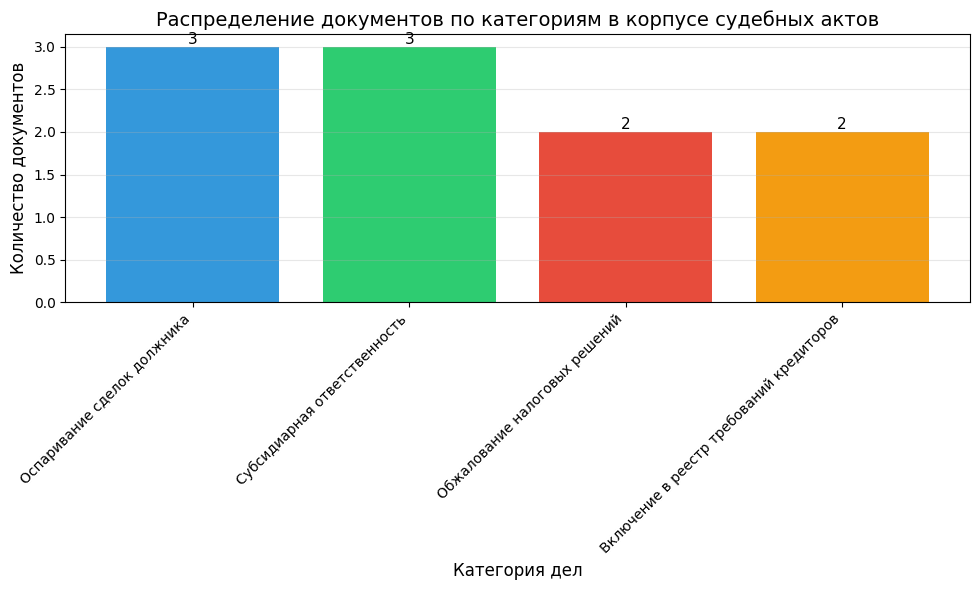
\includegraphics[width=1\textwidth]{../img/result_1.png}
  \caption{Диаграмма распределения документов по категориям}
  \label{fig:category-distribution}
\end{figure}

% \placeholder[Вставьте изображение диаграммы (команда \texttt{\textbackslash includegraphics})]{Рис.~1. Диаграмма распределения документов по категориям}

% \placeholder[Вставьте облако слов по всему корпусу (лемматизированные токены)]{Рис.~2. Облако слов по всему корпусу}

\begin{figure}[h]
  \centering
  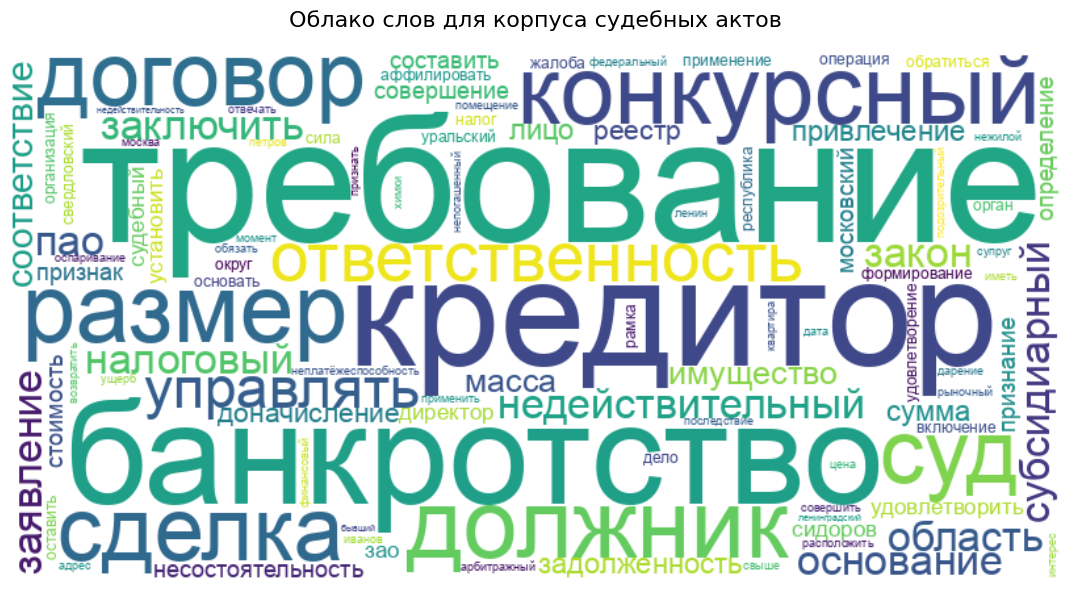
\includegraphics[width=1\textwidth]{../img/result_2.png}
  \caption{Облако слов по всему корпусу}
  \label{fig:category-distribution}
\end{figure}

% \placeholder[Задание 7.3 (повышенная сложность): вставьте облака слов по отдельным категориям]{Рис.~3–6. Облака слов по категориям}

\begin{figure}[h]
  \centering
  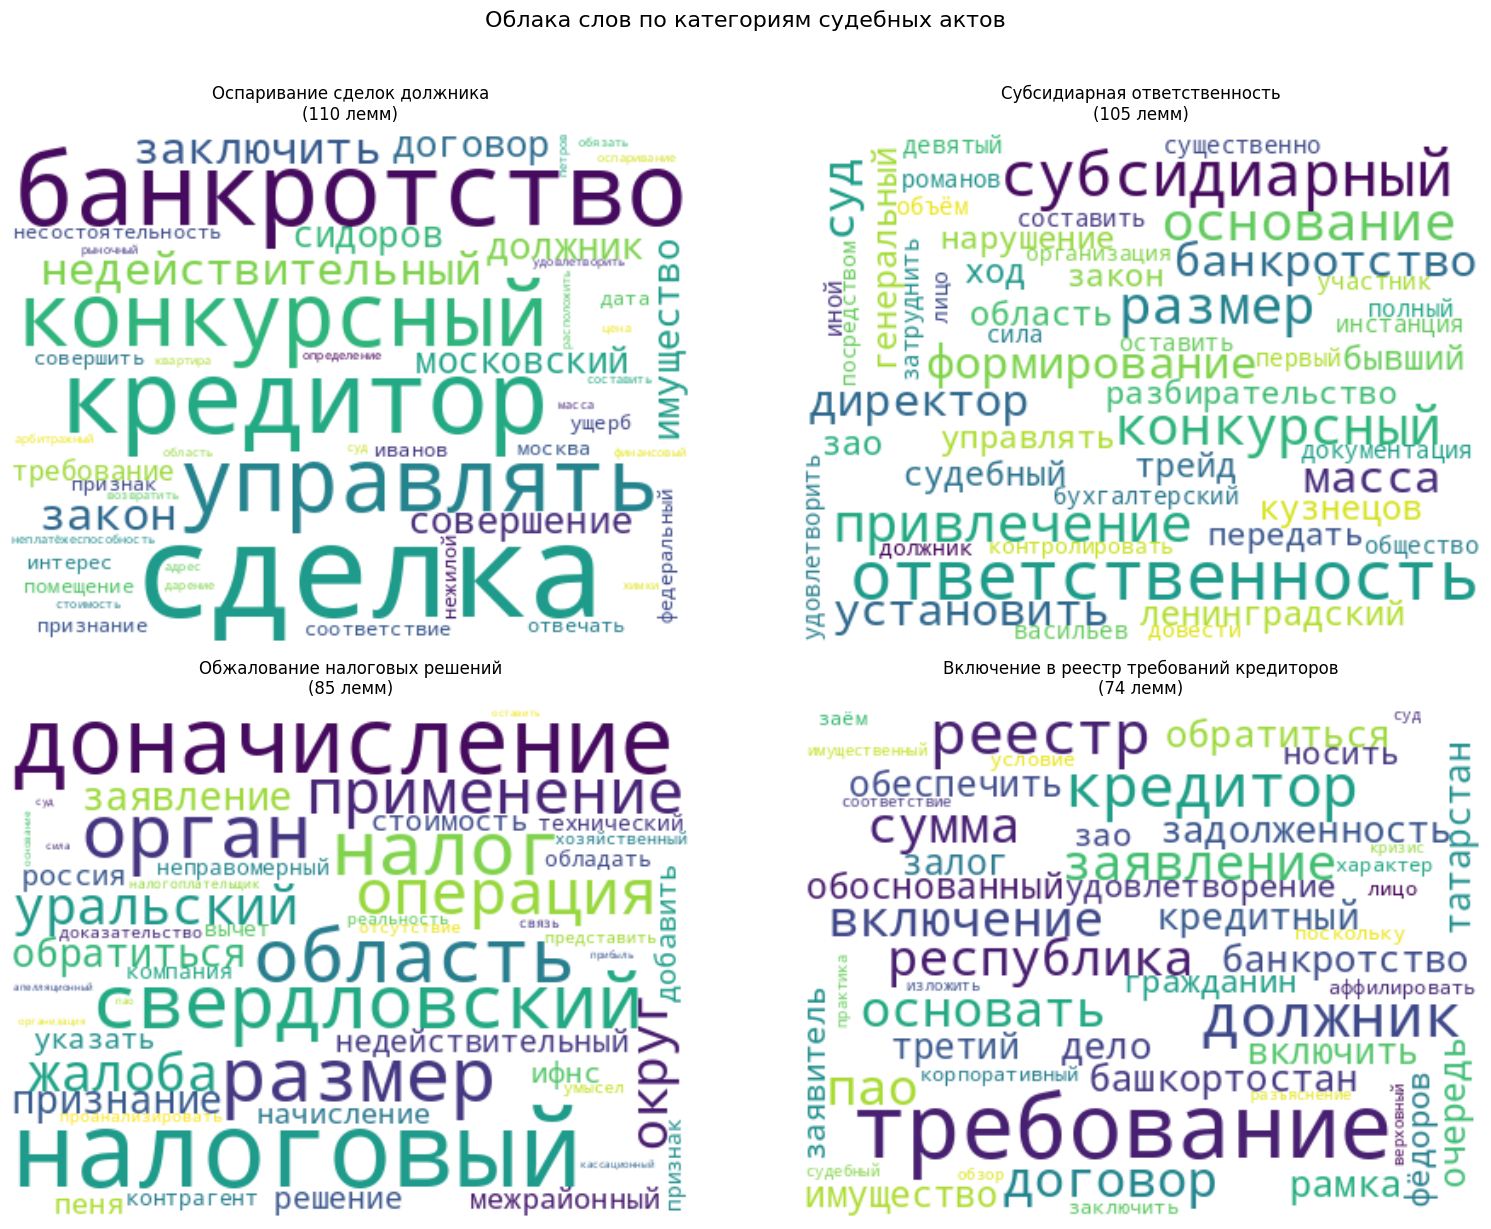
\includegraphics[width=1\textwidth]{../img/result_3.png}
  \caption{Облака слов по категориям}
  \label{fig:category-distribution}
\end{figure}

% ============================================================
%  РАЗДЕЛ 4. КОНТРОЛЬНЫЕ ВОПРОСЫ
% ============================================================
\chapter{Ответы на контрольные вопросы}

\section{Вопрос 1. Лемматизация и стемминг: сравнение}

\textit{Чем лемматизация отличается от стемминга? В каких сценариях предпочтительнее
использование каждого из методов применительно к юридическим текстам?}

\placeholder[Лемматизация приводит слово к его нормальной словарной форме (например, "банкротства" → "банкротство"), тогда как стемминг только отсекает окончания, оставляя основу, которая может не быть реальным словом ("банкротства" → "банкротств"). Для юридических текстов **предпочтительнее лемматизация**, поскольку она точнее работает со сложной морфологией русского языка и сохраняет смысл юридических терминов ("недействительной" → "недействительный", а не "недействительн"). Это критически важно для классификации документов и поиска по ключевым словам, где потеря смысла или неверная нормализация могут привести к искажению результатов анализа. Стемминг может использоваться только при обработке очень больших объемов данных, где скорость важнее точности, или на этапе предварительной фильтрации.]{Ответ на вопрос 1}

\section{Вопрос 2. Стоп-слова и качество классификации}

\textit{Почему удаление стоп-слов улучшает качество классификации текстов? Можно
ли привести пример, когда удаление стоп-слов было бы вредным?}

\placeholder[Удаление стоп-слов улучшает классификацию, поскольку убирает часто встречающиеся служебные слова ("и", "в", "на"), не несущие смысловой нагрузки, что позволяет модели фокусироваться на значимых терминах и снижает размерность признакового пространства. Однако удаление стоп-слов может быть вредным, когда под удаление попадают слова, важные для смысла: например, частица "не" в юридических текстах кардинально меняет смысл ("признал" vs "не признал"). Также в устойчивых юридических оборотах ("в соответствии с", "на основании") удаление предлогов может разрушить ключевые фразы-маркеры определенных категорий документов.]{Ответ на вопрос 2}

\section{Вопрос 3. Ограничения ключевое-словарного классификатора}

\textit{Каковы принципиальные ограничения ключевое-словарного классификатора,
реализованного в Части 6? Какими методами можно преодолеть эти ограничения?}

\placeholder[Ключево-словарный классификатор не учитывает контекст и семантические связи между словами, рассматривая все совпадения как равнозначные. Он требует ручного подбора ключевых слов и плохо масштабируется при увеличении числа категорий. Кроме того, при сильном лексическом пересечении категорий (например, общие термины "банкротство", "кредитор") классификатор может ошибаться, даже если словарь хорошо составлен. Исходя из материалов Лекции 2, для преодоления ограничений ключево-словарного классификатора можно использовать комбинирование нескольких методов извлечения информации (например, анализ статей закона в дополнение к ключевым фразам), а также применять методы машинного обучения на размеченных данных, которые позволяют учитывать контекст и семантические связи между словами, что существенно повышает точность классификации.]{Ответ на вопрос 3}

\section{Вопрос 4. Специализированные библиотеки для русскоязычных текстов}

\textit{Почему для русскоязычных юридических текстов предпочтительно использование
специализированных библиотек, таких как \texttt{natasha}, вместо универсальных
решений?}

\placeholder[Для русскоязычных юридических текстов предпочтительно использование специализированных библиотек вроде Natasha, поскольку они разрабатываются с учетом морфологических особенностей русского языка и показывают высокую точность при работе с юридической лексикой. Исследования подтверждают, что Natasha демонстрирует высокую скорость работы, а в комбинации с другими инструментами позволяет достичь полноценного извлечения сущностей из русскоязычных текстов, что критически важно для анализа судебных актов с их специфической терминологией и структурой.]{Ответ на вопрос 4}

% ============================================================
%  РАЗДЕЛ 5. ИНДИВИДУАЛЬНОЕ ЗАДАНИЕ
% ============================================================
\chapter{Индивидуальное задание}

\section{Добавленные документы}

В данном разделе представлены результаты самостоятельного расширения корпуса
(не менее пяти новых документов).

% \placeholder[Вставьте таблицу: ID\;|\;Категория\;|\;Источник\;|\;Объём (символов)]{Таблица добавленных документов}

\begin{table}[h]
  \centering
  \caption{Таблица добавленных документов}
  \label{table:classification}
  \rowcolors{2}{blue!10}{white}
  \begin{tabular}{l l l r}
  \toprule
  \textbf{ID документа} & 
  \textbf{Категория} & 
  \textbf{Источник} & 
  \textbf{Объём (символов)} \\
  \midrule
  A41-016-2024 & Оспаривание сделок должника & kad.arbitr.ru & 691 \\
  A55-009-2023 & Субсидиарная ответственность & sudact.ru & 605 \\
  A40-011-2024 & Субсидиарная ответственность & КонсультантПлюс & 535 \\
  A40-012-2024 & Субсидиарная ответственность & КонсультантПлюс & 535 \\
  A41-017-2024 & Оспаривание сделок должника & zakon.ru & 535 \\
  \midrule
  \end{tabular}
  \end{table}

\section{Обновлённые результаты классификации}

% \placeholder[Вставьте обновлённую таблицу классификации всех документов]{Результаты классификации расширенного корпуса}

\begin{table}[H]
  \centering
  \caption{Результаты классификации расширенного корпуса}
  \label{tab:classification}
  \rowcolors{2}{LightBlue!30}{white}
  \begin{tabularx}{\textwidth}{l X X c}
    \toprule
    \rowcolor{LightBlue}
    \textsf{\textbf{ID документа}} &
    \textsf{\textbf{Истинная категория}} &
    \textsf{\textbf{Предсказанная категория}} &
    \textsf{\textbf{Верно}} \\
    \midrule
    A40-001-2023 & Оспаривание сделок должника & Оспаривание сделок должника & Да \\
    A40-002-2023 & Оспаривание сделок должника & Оспаривание сделок должника & Да \\
    A56-003-2023 & Субсидиарная ответственность & Субсидиарная ответственность & Да \\
    A56-004-2023 & Субсидиарная ответственность & Субсидиарная ответственность & Да \\
    A60-005-2023 & Обжалование налоговых решений & Обжалование налоговых решений & Да \\
    A60-006-2023 & Обжалование налоговых решений & Обжалование налоговых решений & Да \\
    A07-007-2023 & Включение в реестр требований кредиторов & Включение в реестр требований кредиторов & Да \\
    A07-008-2023 & Включение в реестр требований кредиторов & Включение в реестр требований кредиторов & Да \\
    A40-009-2023 & Оспаривание сделок должника & Оспаривание сделок должника & Да \\
    A40-010-2023 & Субсидиарная ответственность & Субсидиарная ответственность & Да \\
    A41-016-2024 & Оспаривание сделок должника & Оспаривание сделок должника & Да \\
    A55-009-2023 & Субсидиарная ответственность & Субсидиарная ответственность & Да \\
    A40-011-2024 & Субсидиарная ответственность & Субсидиарная ответственность & Да \\
    A40-012-2024 & Субсидиарная ответственность & Субсидиарная ответственность & Да \\
    A41-017-2024 & Оспаривание сделок должника & Оспаривание сделок должника & Да \\
    \midrule
  \end{tabularx}
\end{table}

Обновлённая точность классификатора: \underline{15} /
\underline{15} = \underline{100}\%.

\section{Аналитический вывод}

\placeholder[
  Анализ изменений точности. На исходном корпусе из 10 документов классификатор показал 100\% точность, что объясняется малым объёмом выборки и высокой специфичностью ключевых слов. После расширения корпуса до 15 документов точность сохранилась на уровне 100\% — все новые документы были классифицированы верно. Это свидетельствует об устойчивости предложенного словаря и его способности обобщаться на ранее не встречавшиеся тексты в рамках заданных категорий.

  Выявленные закономерности. Анализ частотности показал, что лемматизация позволила объединить словоформы (сделки → сделка, конкурсного → конкурсный), что повысило статистическую значимость ключевых терминов. NER-анализ выявил характерные ошибки распознавания: модель Natasha корректно определяет коммерческие организации (ООО, ЗАО) и персоны с инициалами, но ошибочно маркирует родовые понятия (Арбитражный суд) как отдельные организации, а также теряет географическую привязку (Уральского округа), которая попадает в категорию LOC.

  Предложения по улучшению словаря. Для повышения робастности классификатора рекомендуется: 1) дополнить словарь более специфичными для категорий терминами, например, для налоговых споров — пени, недоимка, камеральная проверка; 2) исключить из словаря универсальные процессуальные термины (заявление, жалоба, требование), которые присутствуют во всех категориях и создают шум; 3) для повышения точности NER необходимо добавить постобработку, объединяющую полные наименования судов (Арбитражный суд г. Москвы) в единую сущность.
]{Аналитический вывод по индивидуальному заданию}

% ============================================================
%  РАЗДЕЛ 6. ЗАКЛЮЧЕНИЕ
% ============================================================
\chapter{Заключение}

По итогам выполнения лабораторной работы были решены все поставленные задачи.
Реализован полный конвейер предобработки текстовых данных применительно к корпусу
судебных актов, включающий очистку текста, токенизацию, фильтрацию стоп-слов,
лемматизацию и извлечение именованных сущностей. На основе разработанного конвейера
построен ключевое-словарный классификатор и проведена его апробация на учебном корпусе.

\placeholder[
  В ходе выполнения лабораторной работы удалось успешно реализовать полный конвейер обработки текстов и построить классификатор, показавший 100\% точность на расширенном корпусе из 15 документов. Основные затруднения были связаны с подбором стоп-слов для удаления и грамотной аргументацией их выбора — требовалось не просто составить список частотных слов, но и обосновать, почему именно эти леммы не несут смысловой нагрузки для классификации и должны быть исключены. Значительные временные затраты занял анализ результатов работы NER-модуля: выявление ошибок распознавания (например, выделение «Арбитражный суд» как отдельной организации, потеря географической привязки) и их систематизация потребовали детального изучения каждого документа. Для улучшения результатов в будущем целесообразно использовать взвешивание терминов (TF-IDF) вместо простого подсчёта совпадений, а также применить методы машинного обучения на размеченных данных, что позволит учитывать контекст и семантические связи между словами, недоступные при ключево-словарном подходе.
]{Собственные выводы студента}

% ============================================================
%  СПИСОК ЛИТЕРАТУРЫ
% ============================================================
\chapter*{Список литературы}
\addcontentsline{toc}{chapter}{Список литературы}

\begin{thebibliography}{9}
  \bibitem{lec1}
    Материалы Лекции 1 по дисциплине «Информационно-поисковые системы».
    РУДН, 2025.
  \bibitem{lec2}
    Материалы Лекции 2 по дисциплине «Информационно-поисковые системы».
    РУДН, 2025.
  \bibitem{pymorphy2}
    Документация библиотеки \texttt{pymorphy2}.
    URL: \url{https://pymorphy2.readthedocs.io}
  \bibitem{natasha}
    Документация библиотеки \texttt{natasha}.
    URL: \url{https://natasha.github.io}
  \bibitem{nltk}
    Документация библиотеки NLTK (Natural Language Toolkit).
    URL: \url{https://www.nltk.org}
  \bibitem{kad}
    Электронная картотека арбитражных дел.
    URL: \url{https://kad.arbitr.ru}
\end{thebibliography}

% ============================================================
%  ПРИЛОЖЕНИЕ: СВОДНАЯ ВЕДОМОСТЬ БАЛЛОВ
% ============================================================
\chapter*{Приложение. Сводная ведомость баллов}
\addcontentsline{toc}{chapter}{Приложение. Сводная ведомость баллов}
\thispagestyle{plain}

\begin{tcolorbox}[infobox, title={Заполняется преподавателем}]
  \rowcolors{2}{LightBlue!30}{white}
  \begin{tabularx}{\linewidth}{X c c}
    \toprule
    \rowcolor{LightBlue}
    \textsf{\textbf{Критерий оценивания}} &
    \textsf{\textbf{Максимум}} &
    \textsf{\textbf{Получено}} \\
    \midrule
    Часть 2. Очистка текста (Задания 2.1–2.2)          & 20 & \\
    Часть 3. Токенизация и стоп-слова (Задания 3.1–3.2) & 15 & \\
    Часть 4. Лемматизация (Задания 4.1–4.2)             & 15 & \\
    Часть 5. Извлечение сущностей (Задания 5.1–5.2)     & 20 & \\
    Часть 6. Классификация (Задания 6.1–6.2)            & 15 & \\
    Задание 7.3 (повышенная сложность)                  & 15 & \\
    Индивидуальное задание                              & 15 & \\
    \midrule
    \textbf{ИТОГО}                                      & \textbf{100} & \\
    \bottomrule
  \end{tabularx}
\end{tcolorbox}

\vspace{24pt}
\noindent Подпись преподавателя: \underline{\hspace{6cm}}
\\[12pt]
\noindent Дата проверки: \underline{\hspace{4cm}}

\end{document}
